\documentclass[../main.tex]{subfiles}


\begin{document}
%%%%%%%%%%%%%%%%%%%%%%%%%%%%%%%%%%%%%%%%%%%%%%%%%%%%%%%%%%%%%%%%%%%%%%%%%%%%%
%                                                                           %
% Lineare Gleichungssysteme lösen 1: Gausselimination, Lösbarkeitskriterien %
%                                                                           %
%%%%%%%%%%%%%%%%%%%%%%%%%%%%%%%%%%%%%%%%%%%%%%%%%%%%%%%%%%%%%%%%%%%%%%%%%%%%%

\chapter{Lineare Gleichungssysteme lösen 1: Gausselimination, Lösbarkeitskriterien}

\section{Begriffe}
\subsection{Leitkoeffizient}
Den ersten Eintrag einer Zeile, der nicht verschwindet, nennt man Leitkoeffizient (hier eingekreist). \\

$\begin{bmatrix}[ccc|c]
    \circled{2} & 5 & -2 & -3 \\
    \circled{3} & 0 & 1 &  7 \\
    0 & 0 & \circled{8} &  10 \\
\end{bmatrix}$

\subsection{Zeilenstufenform ZFS}
Steht in einer Matrix jeder Leitkoeffizient weiter rechts als der Leitkoeffizient in der Zeile darüber
und stehen alle Zeilen ohne Leitkoeffizient (also solche, in denen nur Nullen stehen) ganz unten,
hat die Matrix die Zeilenstufenform (ZFS). (Hier eingekreist)
\begin{itemize}
    \item Die Leitkoeffizienten müssen nicht zwangsläufig alle auf der Hauptdiagonalen stehen.
    \item Eine quadratische Matrix heisst obere Dreieckmatrix, wenn alle Einträge unter der Hauptdiagonalen Null sind. 
    \item Analog dazu definiert man auch eine untere Dreieckmatrix.
\end{itemize}

$\begin{bmatrix}[cccc|c]
    \circled{2} & 5 & -2 & -1 & -3 \\
    0 & 0 & \circled{3} & -2 &  7 \\
    0 & 0 & 0 & \circled{8} &  10 \\
    0 & 0 & 0 & 0 & 0 \\
\end{bmatrix}$

\subsection{Pivotelemente}
Die Leitkoeffiziente, die man durch Vertauschen der Zeilen möglichst weit links bringt,
nenn man Pivotelemente. \\

$\begin{bmatrix}
    0 & 0 & -1 & 5  \\
    2 & -2 & 1 & 3 \\
    4 & -4 & 3 & 8 \\
\end{bmatrix} \rightarrow$
$\begin{bmatrix}
    \circled{2} & -2 & 1 & 3 \\
    0 & 0 & -1 & 5  \\
    4 & -4 & 3 & 8 \\
\end{bmatrix}$

\section{Gauss-Eliminationsverfahren}
Beim Gauss-Verfahren geht es darum, lineare Gleichungssysteme so umzuformen, dass sich eine
Zeilenstufenform ergibt. Dann wird durch Rückwärtseinsetzen eine eindeutige Lösung bestimmt,
falls das LGS lösbar ist. Dabei geht man Schritt für Schritt vor und wendet in jedem Schritt
eine sogenannte elementare Zeilenstufenform (EZ) auf die EKM (erweiterte Koeffizientenmatrix) an. Davon gibt es drei Typen: \\

\begin{enumerate}
    \item Man darf eine Zeile der EKM  mit einem Faktor, der nicht Nul ist, multiplizieren.
    \item Man darf zwei Zeilen der EKM vertauschen.
    \item Man darf das Vielfache einer Zeile zu einer anderen addieren.
\end{enumerate}

\subsection{Beispiel}
Die EKM (erweiterte Koeffizientenmatrix) ist: \\

$\begin{bmatrix}[ccc|c]
    1 & 2 & 1& 2  \\
    3 & 8 & 1 & 12 \\
    0 & 4 & 1 & 2 \\
\end{bmatrix}$ 
\\ [7pt]
Das daraus resultierende LGS (lineare Gleichungssystem): \\
$x + 2y + z = 2$ \\
$3x + 8y + z = 12$ \\
$ 4y + z = 2$
\\ [7pt]
Im EKS alle Elemente unterhalb der Diagonalen Null bekommen (eingekreist): \\ [7pt]
$\begin{bmatrix}[ccc|c]
    1 & 2 & 1& 2  \\
    \circled{3} & 8 & 1 & 12 \\
    \circled{0} & \circled{4} & 1 & 2 \\
\end{bmatrix}$ 
\\ [7pt]
Zweite Zeile minus drei mal die erste Zeile: \\ [7pt]
$\begin{bmatrix}[ccc|c]
    1 & 2 & 1& 2  \\
    0 & 2 & -2 & 6 \\
    0 & 4 & 1 & 2 \\
\end{bmatrix}$ 
\\ [7pt]
Dritte Zeile minus zwei mal die zweite Zeile: \\ [7pt]
$\begin{bmatrix}[ccc|c]
    1 & 2 & 1& 2  \\
    0 & 2 & -2 & 6 \\
    0 & 0 & 5 & -10 \\
\end{bmatrix}$ 
\\ [7pt]
Zweite Zeile durch 2 dividieren, dritte Zeile durch 5 dividieren: \\ [7pt]
$\begin{bmatrix}[ccc|c]
    1 & 2 & 1& 2  \\
    0 & 1 & -1 & 3 \\
    0 & 0 & 1 & -2 \\
\end{bmatrix}$ 
\\ [7pt]
Nun einfaches LGS auflösen: \\ [7pt]
$x+2y+z=2$ \\
$y-z=3$ \\
$z=-2$ \\
$\Rightarrow z=-2; y=1; x=2$

\section{Lösbarkeit eines LGS}
Bei der Beurteilung der Lösbarkeit von linearen Gleichungssystemen spielt der Rang
zugeordneter Matrizen eine entscheidende Rolle. Der Rang einer Matrix ist eines ihrer
grundlegendsten Merkmale. Es gibt mehrere gleichwertige Definitionen von Rang. Diesen
Begriff werden wir später noch einmal aufnehmen, wenn wir uns mit Verktorräumen
beschäftigen werden.

\subsection{Definition Rang}
Die Anzahl der linear unabhängigen Zeilen oder Spalten einer Matrix A wird einfach als Rang von $\mathbf{A}$ genannt. 
Die Schreibweise ist $r(\mathbf{A})$ \\
Beispiel: \\ [7pt]
$\mathbf{A}= 
\begin{bmatrix}
    1 \;\; 0 \;\; 0  \\
    0 \;\; 1 \;\; 0  \\
    0 \;\; 0 \;\; 1  \\
\end{bmatrix}$
\\ [7pt]
$r(\mathbf{A})=3$ \\ [7pt]
Durch Linearkombination von Zeilen oder Spalten einer Matrix (Multiplikation einer
Zeile/Spalte mit einem Faktor und Addition oder Subtraktion zu einer anderen Zeile/Spalte)
ändert sich der Rang der Matrix nicht. Um den Rang einer Matrix zu bestimmen, formt man
diese daher mittels des Gauss-Verfahrens in eine äquivalente Matrix in Zeilentufenform um:
Wenn die Umformung in einer Zeile stoppt, weil in den nachfolgenden Zeilen nur noch Nullen
stehen, entspricht die Anzahl der Zeilenvektoren, die ungleich Null (0) sind, dann dem Rang der
Matrix.

\subsubsection{Beispiel}
Mittels Eliminationsverfahren die Matrix $\mathbf{A}$ in eine äquivalente Matrix in Zeilenstufenform umformen: \\ [7pt]

$\begin{bmatrix}
    1 & 0 & 1   \\
    -2 & -3 & 1  \\
    3 & 3 & 0 \\
\end{bmatrix} \rightarrow II + I \cdot 2 \rightarrow$
$\begin{bmatrix}
    1 & 0 & 1   \\
    0 & -3 & 3 \\
    3 & 3 & 0 \\
\end{bmatrix} \rightarrow III + I \cdot -2 \rightarrow$ \\ [7pt]

$\begin{bmatrix}
    1 & 0 & 1   \\
    0 & -3 & 3 \\
    0 & 3 & -3 \\
\end{bmatrix} \rightarrow III + II \rightarrow$
$\begin{bmatrix}
    1 & 0 & 1   \\
    0 & -3 & 3 \\
    0 & 0 & 0 \\
\end{bmatrix}$ \\ [7pt]

Die Anzahl der Zeilenvektoren, die ungleich Null (0) sind, entspricht dann dem Rang der Matrix.
Diese Zahl ist hier 2: $r(\mathbf{A})=2$

\subsubsection{Eigenschaften vom Rang}
Seien $n,m \in \mathbb{N}$.
\begin{itemize}
    \item Die einzige Matrix mit Rang 0 ist die Nullmatrix $0_{m\times n}$
    \item Für den Rang einer $(m\times n)-Matrix \mathbf{A}$ gilt: $r(\mathbf{A})<<min(m,n)$.
    \item Die $(n\times n)$-Einheitsmatrix $E_n$ hat den Rang $n$
    \item Die Transponierte $\mathbf{A}^T$ einer Matrix $\mathbf{A}$ hat den selben Rang wie $\mathbf{A}$: $r(\mathbf{A}^T)=r(\mathbf{A})$
    \item Subadditivität: Für zwei $(m\times n)$-Matrizen $\mathbf{A}$ und $\mathbf{B}$ gilt: $r(\mathbf{A}+\mathbf{B}) << r(\mathbf{A}) + r(\mathbf{B})$
\end{itemize}

\subsection{Das Rangkriterium allgemein}
Die EKM ist eine $(m\times(n+1))$-Matrix $[\mathbf{A}|b]$: \\ [7pt]
$[\mathbf{A}|b] = 
\begin{bmatrix}[cccc|c]
    a_{1,1} & a_{1,2} & a_{1,j} & a_{1,n} & b_1 \\
    a_{2,1} & a_{2,2} & a_{2,j} & a_{2,n} & b_2\\
    a_{i,1} & a_{i,2} & a_{i,j} & a_{i,n} & ... \\
    a_{m,1} & a_{m,2} & a_{m,j} & a_{m,n} & b_m \\
\end{bmatrix}$ 

\begin{itemize}
    \item Ist $r(\mathbf{A})=r(\mathbf{A}|b)$, dann hat das GLS eine Lösung, wobei $n-r(\mathbf{A})$ Unbekannten frei gewählt werden können.
    \item Ist $r(\mathbf{A})<r(\mathbf{A}|b)$, dann gibt es keine Lösung.
\end{itemize}

\subsubsection{Beispiele}
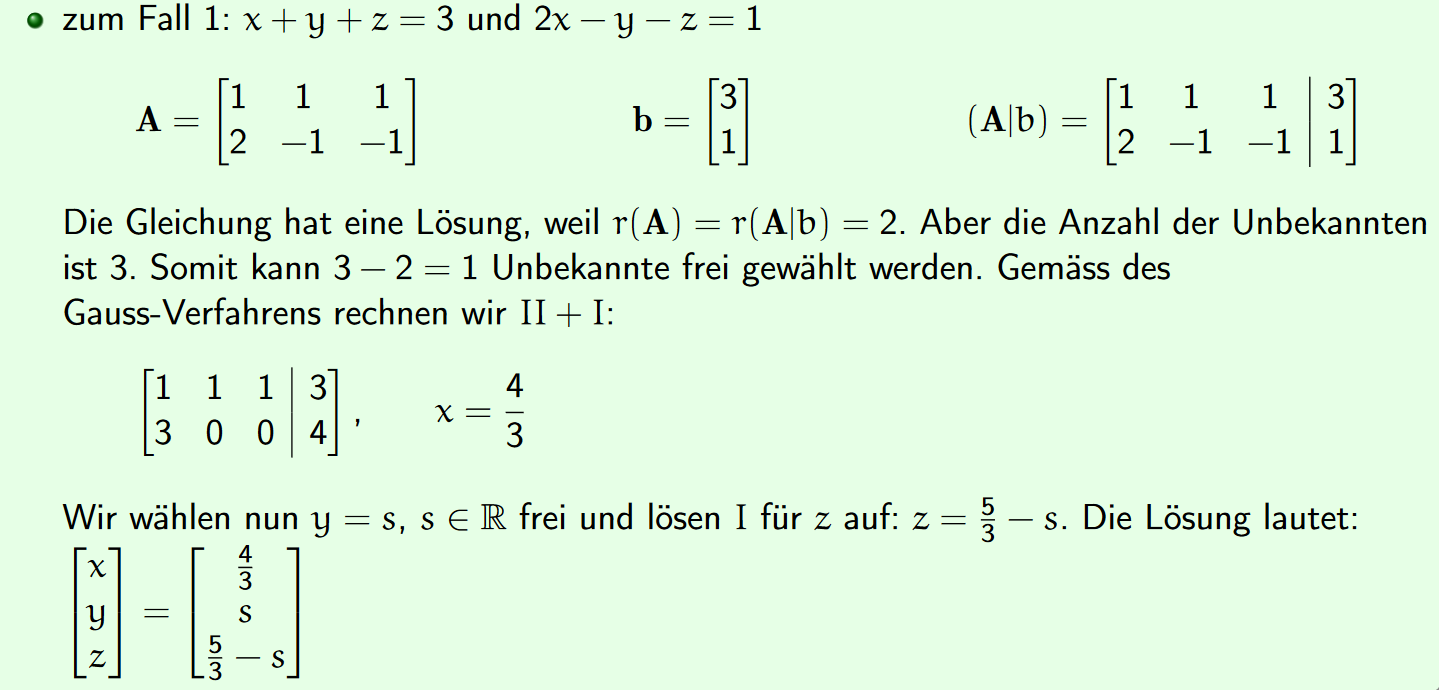
\includegraphics[width=\textwidth,height=\textheight,keepaspectratio]{sw02_rangkriterium_bsp1.PNG} \\ [7pt]
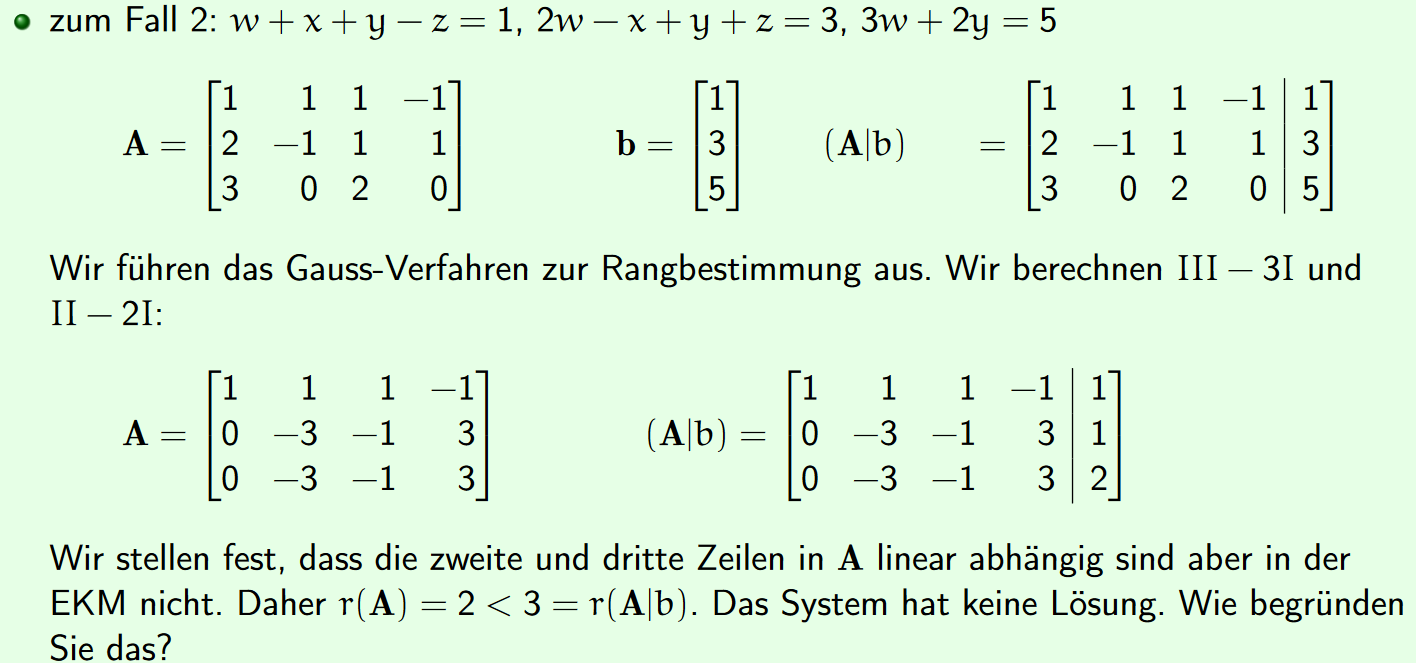
\includegraphics[width=\textwidth,height=\textheight,keepaspectratio]{sw02_rangkriterium_bsp2.PNG}
Wiedersprüchliche Lösung!

\subsection{Rangkriterium im Spezialfall}
Rangkriterium im Speziallfall, nämlich für quadratische $(n\times n)$-Matrizen. 
Das heisst, dass im Folgenden das Gleichungssystem $\mathbf{Ax}=\mathbf{b}$ genau $n$ Unbekannte und $n$ Gleichungen hat.
Dann ist die Koeffizientenmatrix eine $(n\times n)$-Matrix und die EKM eine $(n\times (n+1))$-Matrix. \\
Ein Gleichungssystem $\mathbf{Ax}=\mathbf{b}$ hat:
\begin{itemize}
    \item Genau dann eine eindeutige Lösung, wenn $r(\mathbf{A})=r(\mathbf{A}|b)=n$ gilt. Die Lösung ist dann gegeben durch $\mathbf{x}=\mathbf{A^{-1]}b}$
    \item Unendlich viele Lösungen, wenn $r(\mathbf{A})=r(\mathbf{A}|b)<n$
    \item Keine Lösung, wenn $r(\mathbf{A})<r(\mathbf{A}|b)$
\end{itemize}

\subsubsection{Beispiele}
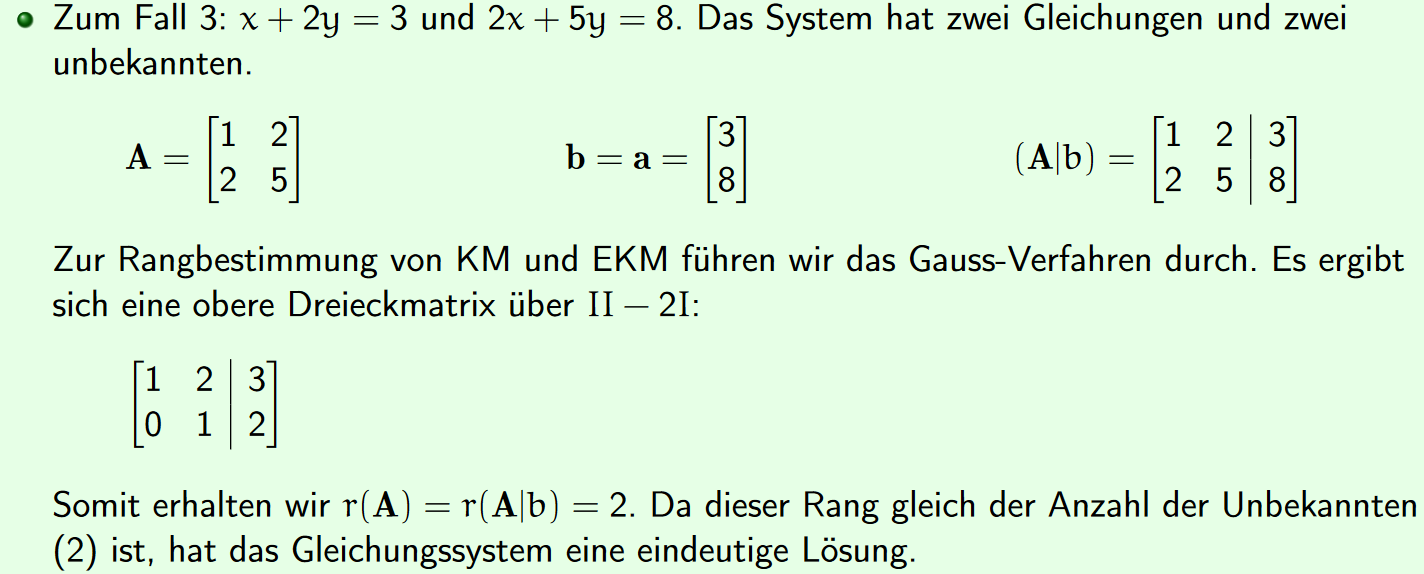
\includegraphics[width=\textwidth,height=\textheight,keepaspectratio]{sw02_rangkriterium_bsp3.PNG} \\ [7pt]
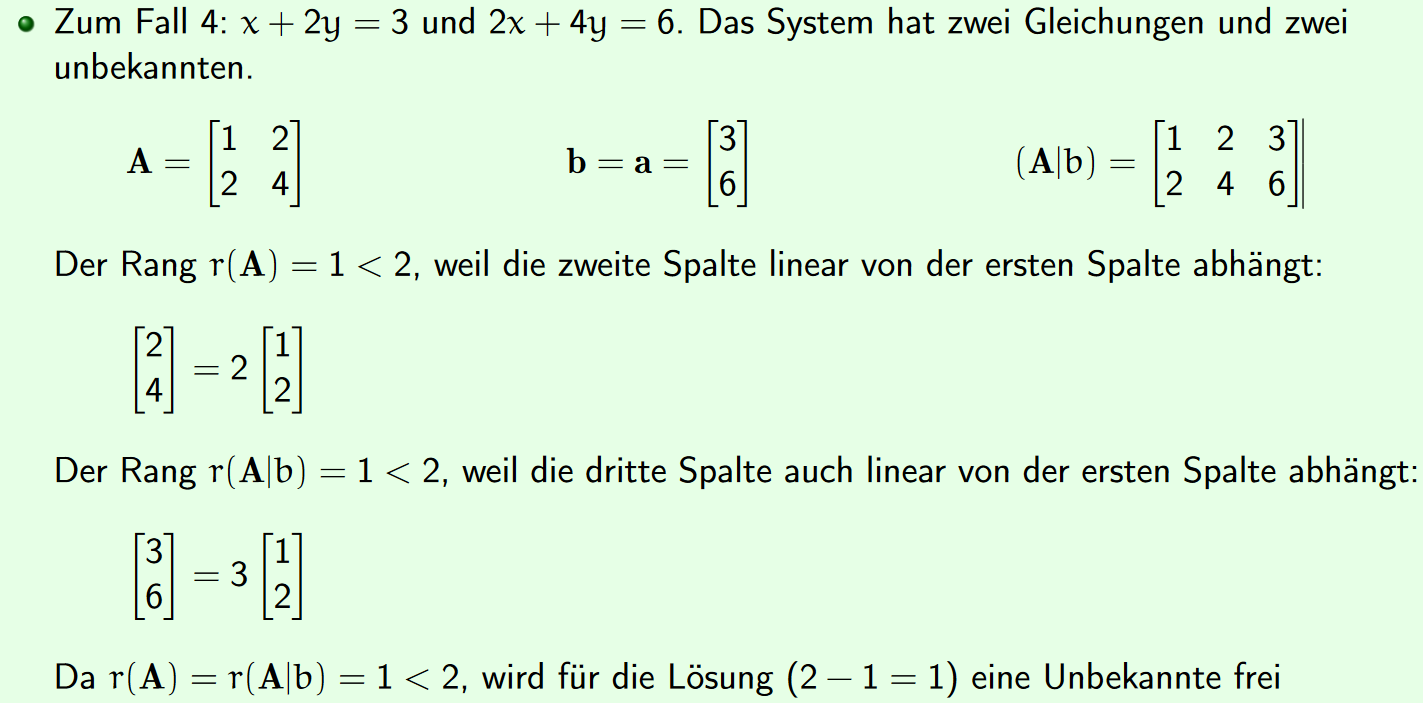
\includegraphics[width=\textwidth,height=\textheight,keepaspectratio]{sw02_rangkriterium_bsp4.PNG} \\
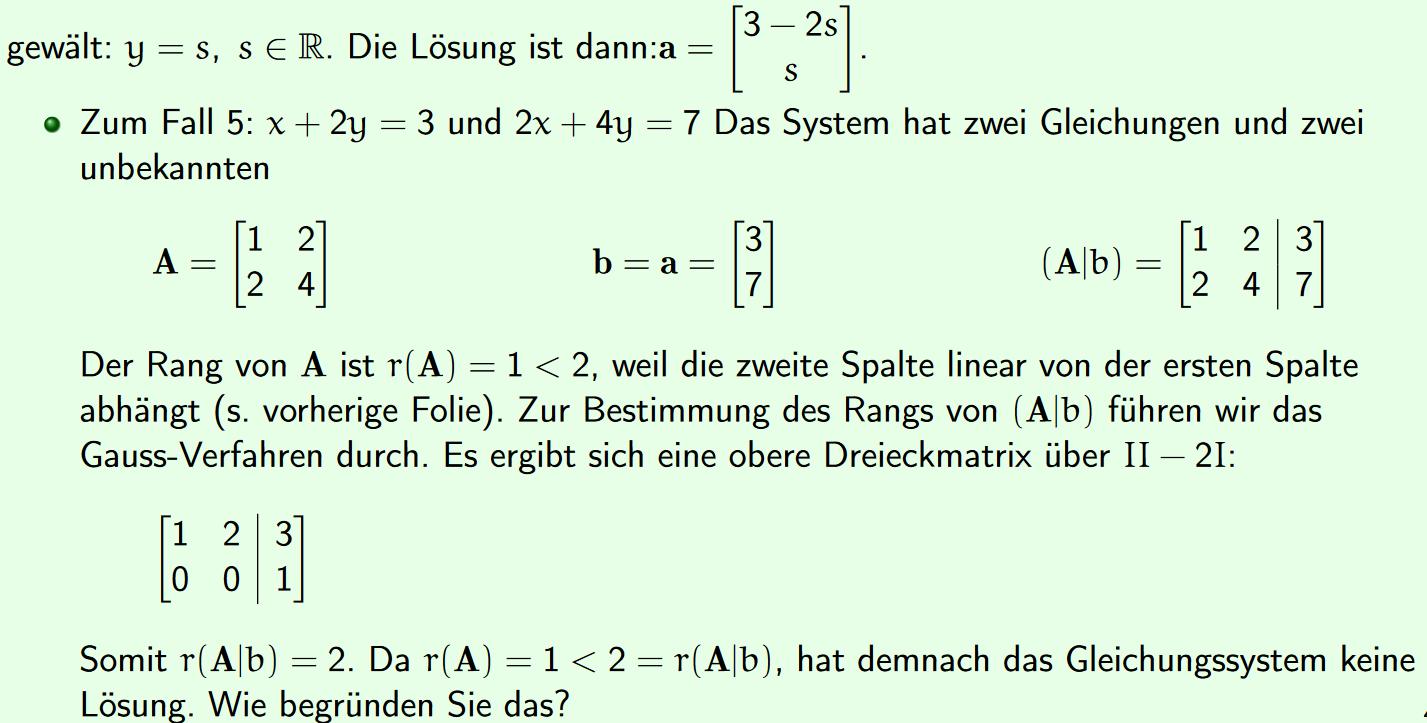
\includegraphics[width=\textwidth,height=\textheight,keepaspectratio]{sw02_rangkriterium_bsp5.PNG}

\section{Schlüsselergebnisse}
\begin{itemize}
    \item Das Gauss-Verfahren bringt Koeffizientenmatrix und erweiterte Koeffizientenmatrix der linearen Gleichungssysteme in Zeilenstufenform.
    \item Das Endergebnis des Gauss-Verfahren ist in der Regel eine obere oder untere Dreieckmatrix.
    \item Das Gauss-Eliminationsverfahren ändert die Lösungen der ursprünglichen Matrix nicht.
    \item Das Gauss-Eliminationsverfahren ändert die Anzahl der linear unabhängigen Zeilen oder Spalten nicht.
    \item Für den Rang einer $(m\times n)$-Matrix $\mathbf{A}$ gilt: $r(\mathbf{A})<<min(m,n)$
    \item Für LGS $\mathbf{Ax}=\mathbf{b}$ mit $n$ Gleichungen und $n$ unbekannten, ist $\mathbf{A}$ eine quadratische $(n\times n)$-Matrix. 
    Wenn $r(\mathbf{A})=r(\mathbf{A}|b)=n$, dann hat das GLS eine eindeutige Lösung, die durch $\mathbf{x}=\mathbf{A^{-1}b}$ gegeben ist.
    \item Ist der Rang einer quadratischen Matrix gleich ihrer Zeilen- und Spaltenzahl, hat sie vollen Rang und ist regulär (invertierbar).
\end{itemize}







\end{document}